

    而后将始终只考虑这种定向的正交归一基。

一个具有确定指向的、时间定向的正交基就是\textit{惯性基矢},由于矢量空间和闵氏背景本身的等同,我们就可以把这些矢量都“搬”到闵氏时空里来。

一般认为所考虑的惯性系(进而惯性基矢)都应具备一致时间定向。
    


惯性坐标系一般就选择处处与参考系标架一致的坐标基,可统称惯性系。

因为参考系由充斥于时空(或其开子集)的无数观者组成,过每一时空点有且仅有一条观者世界线,所以,给定一个参考系后,全时空(或其开子集)就有一个 4-标架场。任何时空点的任何张量都可用该点的4-标架作为基底表出。
\begin{definition}[观者]
    观者指一条定义了4-标架场 $\{e_\mu\}$ 的类时世界线,并规定
    \eq{
    g(e_\mu,e_\nu)=\eta_{\mu\nu},\quad e_0=Z.
    }
    这里 $g$ 是时空所配度规,闵氏时空取 $\upeta$。
\end{definition}
世界线为测地线的运动就称为\textit{惯性运动},则对惯性观者的准确定义是:
\begin{definition}[惯性观者]
    惯性观者是做惯性运动的无自转观者。
\end{definition}

决定一个瞬时观者的要素除 $p,Z$外,有时还要辅以 3-标架,它们与 $Z$ 组成$p$点的正交4-标架$\{e_\mu\}$,在此情况下一个瞬时观者应表为
\[(p,\{e_\mu\}),\]
其中 $e_0=Z$。不必强调标架时,瞬时观者仍可表为$(p,Z)$。


关键在于何种情况不仅使得保内积,还使得轴“不动”。不妨这样设想,非测地线意味着 3-速在变化,进而一点的瞬时观者可 boost 到邻近点的另一瞬时观者去,这样,此点观者所持的空间矢量便自然能延至下一观者中去。boost 变换下,$e_\mu$ 间当然能保持正交,说明各点瞬时观者或 4-标架场各点取值间差的正是\textit{无穷小(infinitesimal) boost 变换}。将非测地线看作是一系列瞬时惯性观者的无穷小 boost 变换,轻松使得 $e_i$ 保持其空间性。并且,由于点之间接近,boost 也不包含空间转动(只受 3-速影响),故各 $e_i$ 朝向不变。

$Z,A$ 正交使得 $Z$ 保模长地发生“转动”,因而空间矢量为与之正交而一齐转动。这种转动只涉及到 $Z,A$ 所在(无穷小)平面,此即,boost 变换应是关于 $Z,A$ 平面的伪转动。3 维空间中旋转变换是相关于一个角速度矢量而言的,即
\eq{
\dv{v_i}{\tau}=(\vec\omega\times\vec v)^i=\varepsilon_{ijk}\omega^j v^k,
}
其同时可看作处于 $\vec\omega$ 所对平面上的旋转(按右手螺旋),这个视角在代数上就是在 3 维空间中取其对偶的 2-形式(当然,先用旋转平面的诱导度规降下来),即 $\Omega=\star\vec\omega$,分量为 $\Omega_{ik}=\omega^j\varepsilon_{jik}=-\omega^j\varepsilon_{ijk}$。这样
\eq{
\dv{v^i}{\tau}=(\vec\omega\times\vec v)^i=-\Omega^{ij} v_j,
}
这里旋转平面的特点是同 $\vec\omega$ 垂直,这意味着 $\vec\omega$ 正比于平面上任二线性无关矢量之叉乘,则 $\Omega$ 正比于其楔积。将其推广至高维时,旋转平面有其确切含义(找到两个线性无关矢量),而角速度矢量的对偶不再是平面,故表述上采取 2-形式而非矢量叉乘:
\eq{
\dv{v^\mu}{\tau}=-\Omega^{\mu\nu} v_\nu,
}
此处应将 $\dv*{\tau}$ 理解为惯性坐标系的$D/\d\tau$,而 $\Omega$ 正比于 $A\wedge Z$。令 $v=Z$,则
\[
-\Omega^{\mu\nu} Z_\nu\propto -(A^\mu Z^\nu-Z^\mu A^\nu)Z_\nu=A^\mu=-\Omega^{\mu\nu} Z_\nu.
\]
说明比例系数归一。上式移项后所定义的导数,便满足我们对费移 $D_F v/\d\tau=0$ 的要求。

综上,无自转观者所要求的无非是 4-标架沿线费移。以后谈及等效原理会详述无自转的重要性,如可以避开科氏惯性力之干扰。

\begin{wrapfigure}{l}{.35\textwidth}
    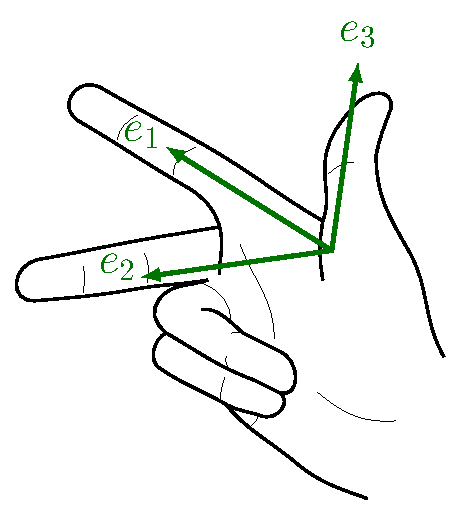
\includegraphics[width=.3\textwidth]{fig/chpt01/tetrad hand.pdf}
    \caption{空间右手 3-标架}
\end{wrapfigure}
还需处处配以\textit{4-标架(tetrad)},也即其上任意点矢量的正交归一基 $\{\bm{e}_\mu\}$,满足 $\bm{e}_\mu\cdot\bm{e}_\nu=\eta_{\mu\nu}$。直观上,\textit{3-标架(frame)}可以是由三根单位长的短直杆或刻度尺焊成的正交架子,每根直杆代表一个观测方向,其在每一时刻的指向由该观者选定。读者亦可尝试用右手大拇指、食指及中指按右手螺旋比划出 3-标架。数学上,3-标架就是空间正交归一基 $\{\bm{e}_i\}$,“空间”指皆与观者世界线切矢 $\bm{e}_0$ 正交。今后谈及 4-标架时默认为右手标架。



因而 4-标架场又称作观者所处处配备的“局部实验室”,所测物理量无非就是将相关的 4 维量投影到 3-标架上。


惯性观者的 4-标架又称\textit{惯性基矢}或\textit{惯性标架}。我们还应希望惯性标架\textit{无自转},否则可能观测到赝力。如图 \ref{k&c},设 Cynthia、Kaylor 两人坐在地面的两把椅子上:Cynthia 坐底座固定的蛋壳椅;Kaylor 坐底座静置的办公椅且不停自转。二者世界线都走直线,但 Cynthia 可视为惯性观者而 Kaylor 不能。
\begin{figure}%
    \centering
    \subfloat[\centering Cynthia]{{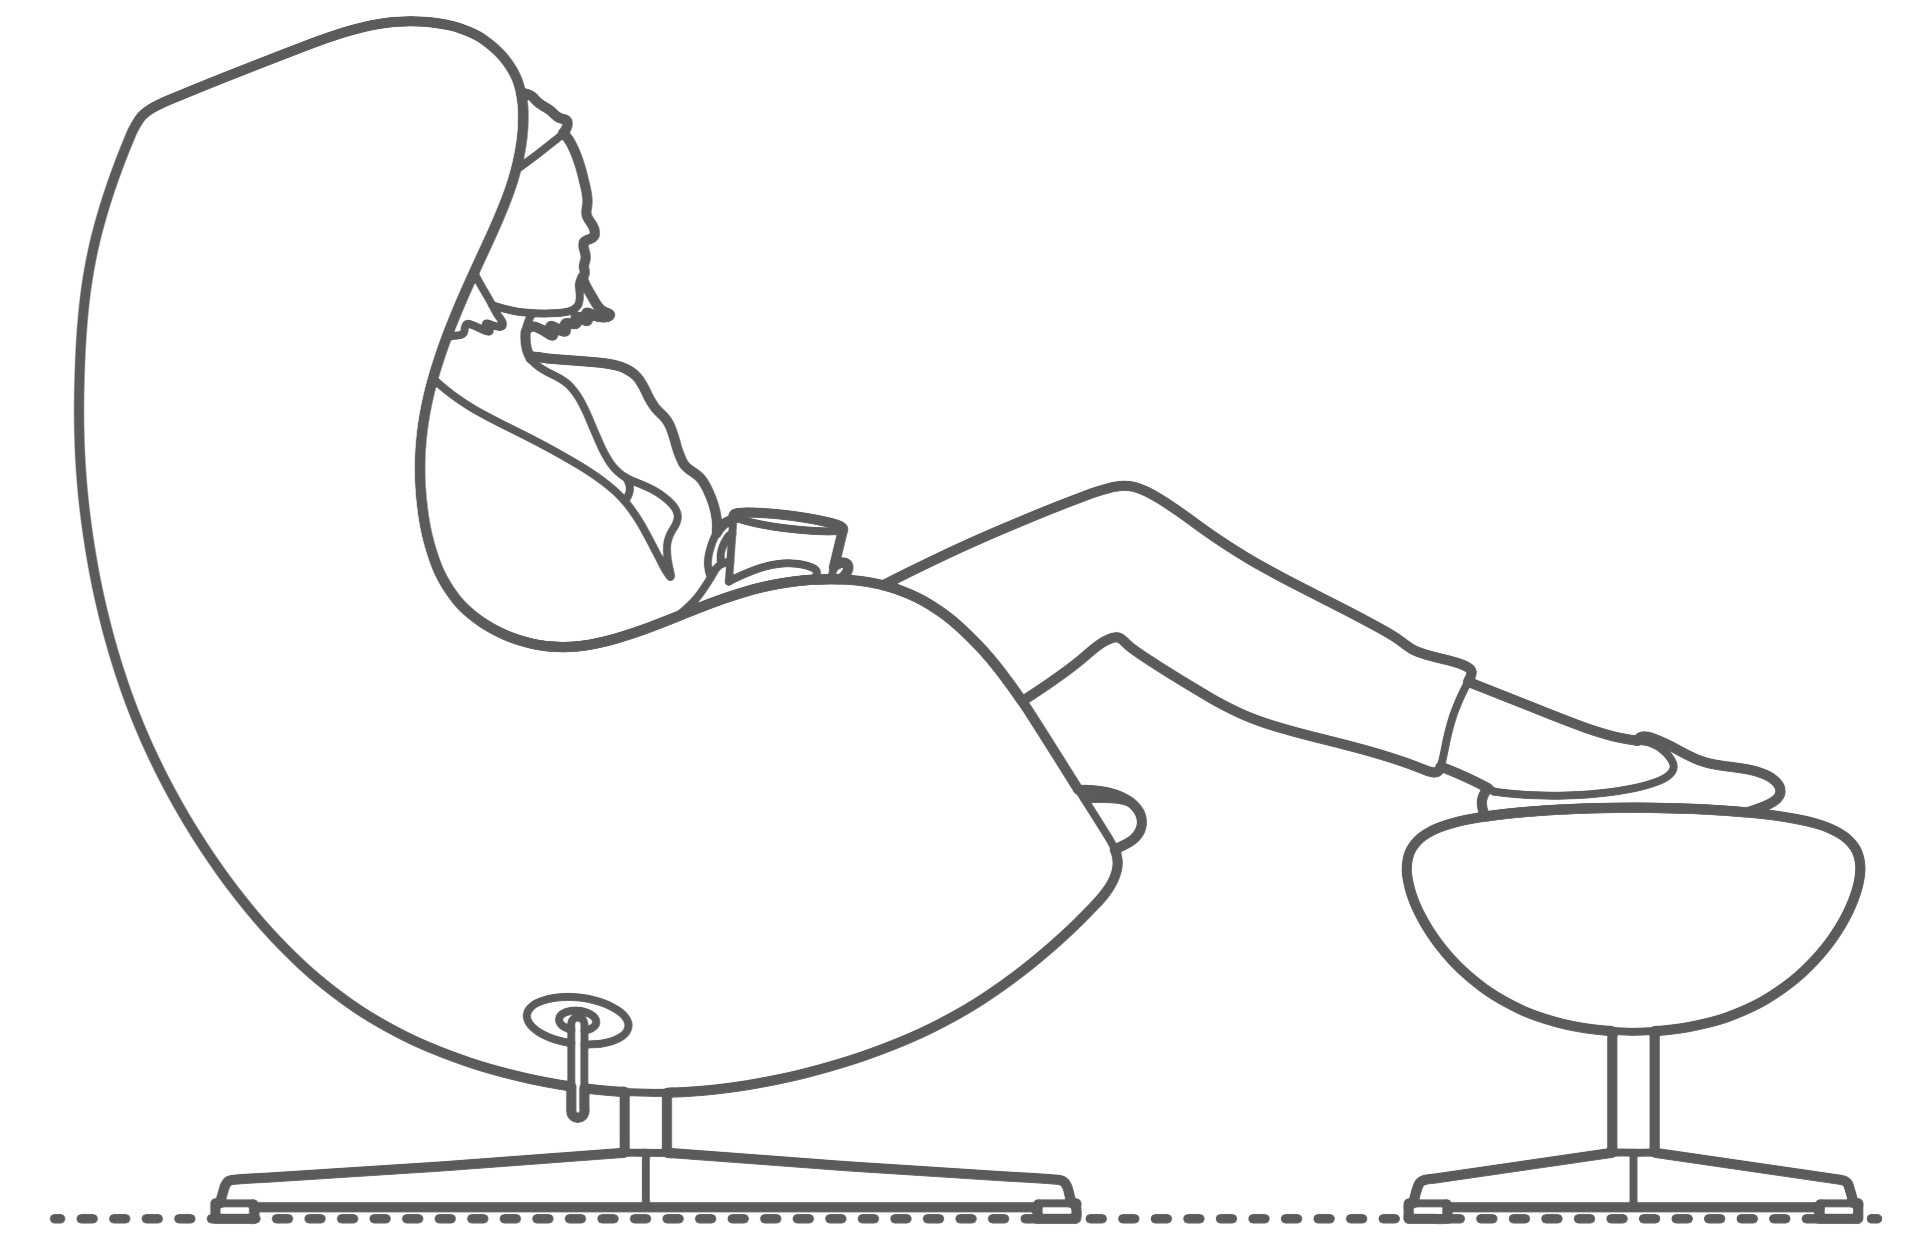
\includegraphics[width=.5\textwidth]{fig/chpt01/eggchair.jpg} }}%
    \subfloat[\centering Kaylor]{{
\tikzset{every picture/.style={line width=0.75pt}} %set default line width to 0.75pt        
\begin{tikzpicture}[x=0.75pt,y=0.75pt,yscale=-.73,xscale=.73]
%uncomment if require: \path (0,300); %set diagram left start at 0, and has height of 300
%Image [id:dp40969400488164953] 
\draw (147,147) node  {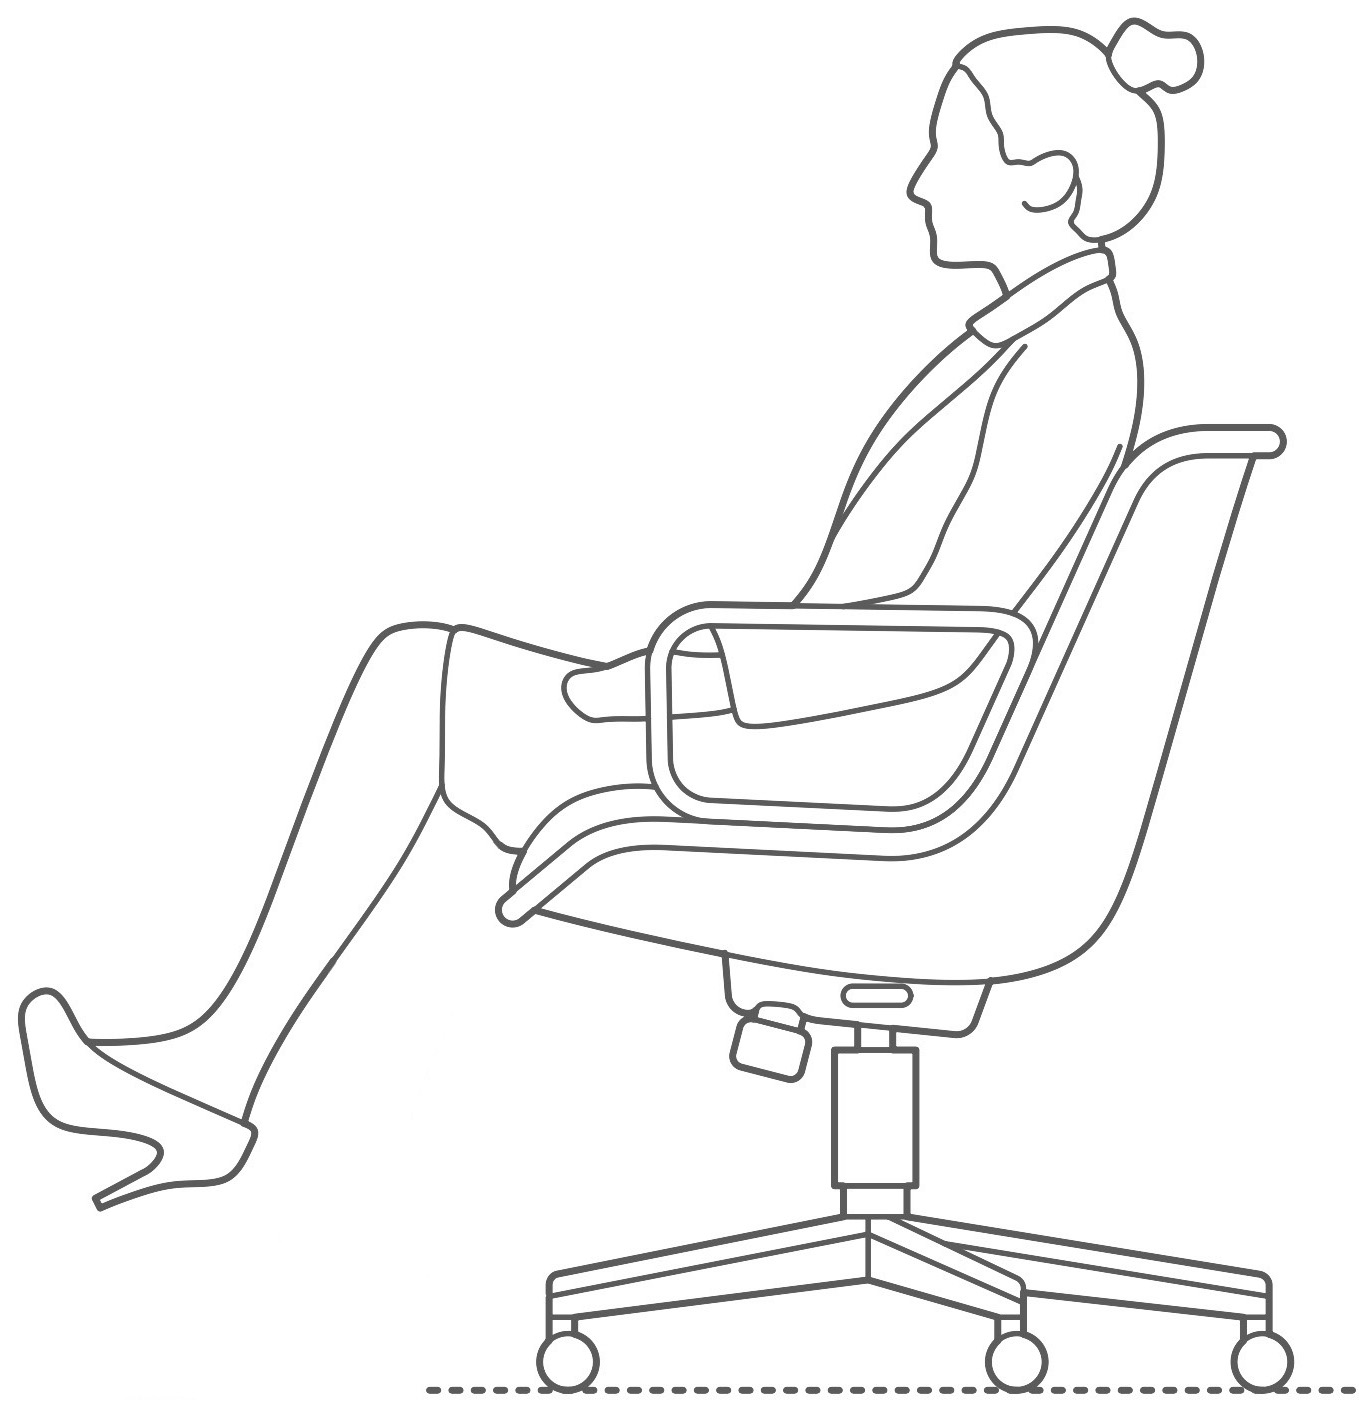
\includegraphics[width=.38\textwidth]{fig/chpt01/rolling.jpg}};
%Shape: Arc [id:dp1232081022977285] 
\draw  [draw opacity=0] (185.25,85.75) .. controls (185.23,85.75) and (185.22,85.75) .. (185.21,85.75) .. controls (142.38,85.75) and (107.67,76.44) .. (107.67,64.96) .. controls (107.67,53.48) and (142.38,44.17) .. (185.21,44.17) .. controls (187.04,44.17) and (188.85,44.18) .. (190.65,44.22) -- (185.21,64.96) -- cycle ; \draw  [thin,color={rgb, 255:red, 128; green, 128; blue, 128 }  ,draw opacity=1 ] (185.25,85.75) .. controls (185.23,85.75) and (185.22,85.75) .. (185.21,85.75) .. controls (142.38,85.75) and (107.67,76.44) .. (107.67,64.96) .. controls (107.67,53.48) and (142.38,44.17) .. (185.21,44.17) .. controls (187.04,44.17) and (188.85,44.18) .. (190.65,44.22) ;  
%Shape: Arc [id:dp5238961792452044] 
\draw  [draw opacity=0] (248.09,128.99) .. controls (233.93,134.01) and (211.48,137.25) .. (186.21,137.25) .. controls (143.38,137.25) and (108.67,127.94) .. (108.67,116.46) .. controls (108.67,105.37) and (141.02,96.32) .. (181.78,95.7) -- (186.21,116.46) -- cycle ; 
\draw  [thin,color={rgb, 255:red, 128; green, 128; blue, 128 }  ,draw opacity=1 ] (248.09,128.99) .. controls (233.93,134.01) and (211.48,137.25) .. (186.21,137.25) .. controls (143.38,137.25) and (108.67,127.94) .. (108.67,116.46) .. controls (108.67,105.37) and (141.02,96.32) .. (181.78,95.7) ;  
%Shape: Arc [id:dp16124070044095484] 
%\draw  [draw opacity=0] (236.4,198.46) .. controls (252.27,202.27) and (262.25,207.8) .. (262.25,213.96) .. controls (262.25,225.44) and (227.53,234.75) .. (184.71,234.75) .. controls (141.88,234.75) and (107.17,225.44) .. (107.17,213.96) .. controls (107.17,206.9) and (120.29,200.66) .. (140.35,196.9) -- (184.71,213.96) -- cycle ; 
%\draw  [thin,color={rgb, 255:red, 128; green, 128; blue, 128 }  ,draw opacity=1 ] (236.4,198.46) .. controls (252.27,202.27) and (262.25,207.8) .. (262.25,213.96) .. controls (262.25,225.44) and (227.53,234.75) .. (184.71,234.75) .. controls (141.88,234.75) and (107.17,225.44) .. (107.17,213.96) .. controls (107.17,206.9) and (120.29,200.66) .. (140.35,196.9) ;  
%Shape: Arc [id:dp3765315090738246] 
\draw  [draw opacity=0] (254.35,155.08) .. controls (259.1,157.78) and (261.75,160.78) .. (261.75,163.96) .. controls (261.75,175.44) and (227.03,184.75) .. (184.21,184.75) .. controls (166.81,184.75) and (150.76,183.21) .. (137.82,180.62) -- (184.21,163.96) -- cycle ; 
\draw  [thin,color={rgb, 255:red, 128; green, 128; blue, 128 }  ,draw opacity=1 ] (254.35,155.08) .. controls (259.1,157.78) and (261.75,160.78) .. (261.75,163.96) .. controls (261.75,175.44) and (227.03,184.75) .. (184.21,184.75) .. controls (166.81,184.75) and (150.76,183.21) .. (137.82,180.62) ;  
%Shape: Arc [id:dp2760353626475096] 
\draw  [draw opacity=0] (245.35,51.83) .. controls (256.23,55.41) and (262.75,59.98) .. (262.75,64.96) .. controls (262.75,73.17) and (244.98,80.28) .. (219.17,83.65) -- (185.21,64.96) -- cycle ; \draw  [thin,color={rgb, 255:red, 128; green, 128; blue, 128 }  ,draw opacity=1 ] (245.35,51.83) .. controls (256.23,55.41) and (262.75,59.98) .. (262.75,64.96) .. controls (262.75,73.17) and (244.98,80.28) .. (219.17,83.65) ;  
\end{tikzpicture}
    }}%
    \caption{\small Cynthia 可视为惯性观者而 Kaylor 不能}\label{k&c}
\end{figure}
请注意,虽然观者概念本身已要求把此二人看成没有大小的点(于是由一世界线代表),但自转涉及的仅是线上各点每一空间基矢的方向沿线是否改变,故仍有明确意义。然而在惯性观者所对应的惯性坐标系中,若令 4-标架 $\{\bm{e}_\mu\}$ 就是相应的坐标基,则直观看来就是无自转的。一般默认将 4-标架取为惯性坐标基。借助惯性坐标系便可定量地定义无自转观者。




瞬时观测




测地线切矢就是时间轴的方向,那么与之正交就代表着空间方向,


动力学